\chapter{Stereo Matching}
\label{ch:lesson22}

Two cameras viewing the same scene from slightly different positions see the same 3D points shifted by different amounts depending on depth --- nearby points shift more, distant points shift less. \textbf{Stereo matching} finds these shifts (the \textbf{disparity}) at every pixel, which convert into depth via triangulation. The key problem is correspondence: finding, for every pixel in the left image, the matching pixel in the right. This chapter builds a \textbf{block matcher} that solves it by comparing small patches with sum-of-squared differences (SSD) --- a close cousin of Chapter~\ref{ch:lesson21}'s optical flow, but restricted to a 1D search along a single row instead of a full 2D neighborhood.

\section{Rectified stereo: why the search is 1D}

For a pair of cameras that are side-by-side, pointed the same direction, with parallel image planes (a \textbf{rectified} stereo pair --- real camera rigs are calibrated and warped to approximate this), a fundamental fact of epipolar geometry applies: the corresponding point for any pixel in the left image lies \textbf{on the same row} in the right image. This collapses the search from a 2D image search down to a 1D scan along one row, and the horizontal offset between the two matching positions is the \textbf{disparity} $d$.

Disparity relates to depth by
\begin{equation}
Z = \frac{f \cdot B}{d},
\end{equation}
where $f$ is the focal length and $B$ is the baseline (distance between the two camera centers). For a rectified pair, depth is \textbf{inversely proportional to disparity}: nearby objects have large disparity, distant objects have small disparity, and an object infinitely far away has zero disparity.

\section{A synthetic stereo pair with known ground truth}

A left image of pure random texture (so every patch is locally distinctive --- no aperture-problem ambiguity), with a right image constructed by shifting each pixel left by its true disparity, set to three different constant values for three depth ``planes'': a background and two nearer rectangles. Nearer surfaces uncover background pixels that have no corresponding pixel in the left image at all --- an \textbf{occlusion}, patched with fresh random noise. Figure~\ref{fig:l22-1} shows the resulting stereo pair and ground truth.

\begin{figure}[h]
\centering
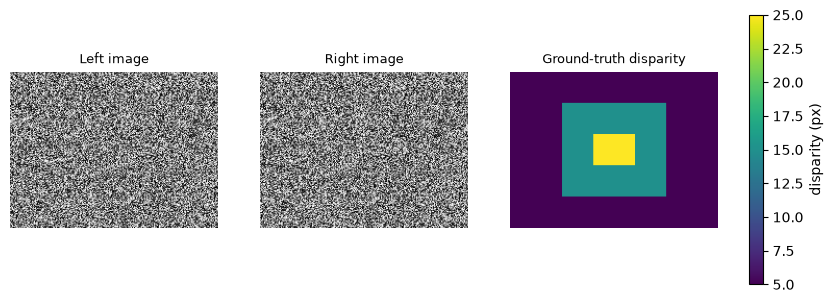
\includegraphics[width=0.9\textwidth]{figures/lesson22_fig01.png}
\caption{Left image, right image, and ground-truth disparity (three depth planes).}
\label{fig:l22-1}
\end{figure}

\section{Block matching along the scanline}

For each pixel in the left image, slide a small window along the \emph{same row} of the right image over a range of candidate disparities and keep the disparity with the lowest sum-of-squared-differences.

\begin{lstlisting}
for d in range(max_disp + 1):
    xr = x - d
    right_patch = right_f[y-half:y+half+1, xr-half:xr+half+1]
    cost = ((left_patch - right_patch)**2).sum()
    if cost < best_cost:
        best_cost, best_d = cost, d
\end{lstlisting}

\begin{figure}[h]
\centering
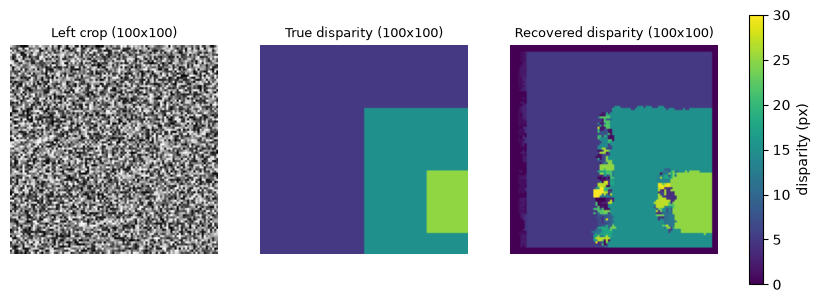
\includegraphics[width=0.9\textwidth]{figures/lesson22_fig02.png}
\caption{A $100\times100$ crop, its true disparity, and the recovered disparity from a from-scratch block matcher --- the three depth planes are cleanly separated away from the border and depth-boundary regions.}
\label{fig:l22-2}
\end{figure}

As Figure~\ref{fig:l22-2} shows, within the interior of the rectangles, the recovered disparity matches the ground truth almost perfectly (mean disparity $5.03$, $15.03$, $25.04$ against true values $5$, $15$, $25$). The exception is the speckled band at each rectangle's edge: a window straddling a depth boundary mixes pixels from two different true disparities, so no single candidate disparity fits the whole window well --- a preview of the occlusion problem tackled next.

\section{Catching bad matches: the left-right consistency check}

Occlusions and depth-boundary ambiguity produce wrong matches, like the speckle above. The fix: match both left-to-right and right-to-left, then keep only the pixels where the two results agree, discarding the rest as unreliable. Computing the right-to-left disparity needs no new code --- flip both images left-right, swap which one plays ``left,'' run the exact same matcher, then flip the result back. Figure~\ref{fig:l22-3} shows both directions and the consistency result.

\begin{figure}[h]
\centering
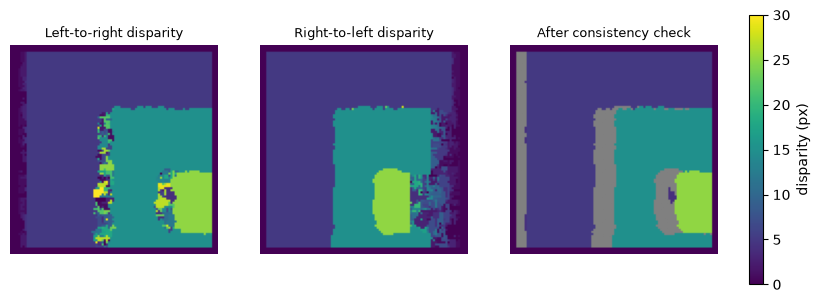
\includegraphics[width=0.9\textwidth]{figures/lesson22_fig03.png}
\caption{Left-to-right disparity, right-to-left disparity, and the result after the consistency check (gray = rejected). On this crop, $1440$ of $10{,}000$ pixels are marked inconsistent, concentrated at occlusions and depth-boundary windows.}
\label{fig:l22-3}
\end{figure}

\section{The same thing, at full resolution, with OpenCV}

\code{cv2.StereoBM} implements this same block-matching idea (with efficiency and post-processing refinements) fast enough to run on the whole image. \code{StereoBM} marks a pixel invalid wherever it isn't confident in a unique match, e.g.\ too close to the image border to search the full disparity range, as Figure~\ref{fig:l22-4} shows.

\begin{figure}[h]
\centering
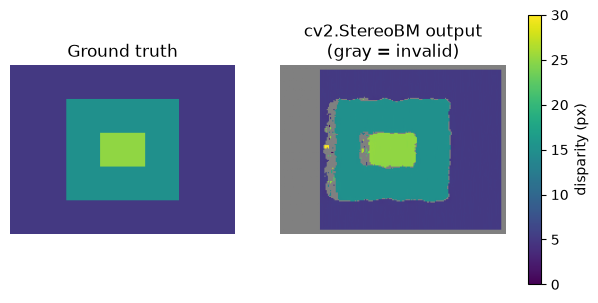
\includegraphics[width=0.7\textwidth]{figures/lesson22_fig04.png}
\caption{Ground truth vs.\ \code{cv2.StereoBM} output at full resolution (gray = invalid).}
\label{fig:l22-4}
\end{figure}

The left-right consistency check is also built into \code{cv2.StereoBM} --- set \code{disp12MaxDiff} to a small positive number (typically 1) to enable it. On the full synthetic image: $21{,}706$ valid pixels without the check, $21{,}442$ with it --- $264$ pixels newly flagged invalid.

\section{Window size: detail vs.\ noise tradeoff}

A larger matching window averages over more pixels, making the match more robust to noise but blurring across depth discontinuities. A smaller window preserves sharp depth boundaries but is more easily fooled by noise or repetitive texture, as Figure~\ref{fig:l22-5} shows.

\begin{figure}[h]
\centering
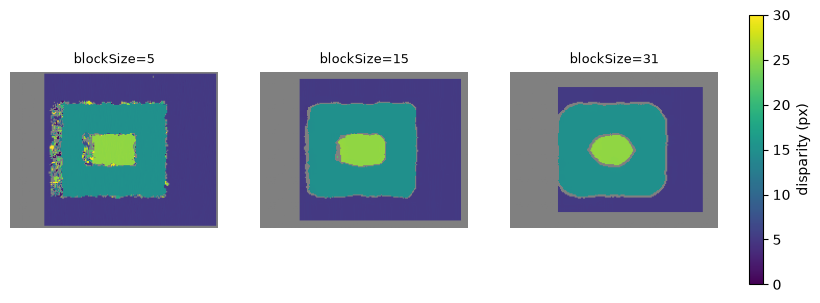
\includegraphics[width=0.9\textwidth]{figures/lesson22_fig06.png}
\caption{\code{blockSize} 5, 15, and 31 on the same stereo pair --- small windows preserve sharp edges but are noisier; large windows are smoother but blur depth boundaries.}
\label{fig:l22-5}
\end{figure}

\section{A real stereo pair: Tsukuba}

Everything so far has used synthetic images, precisely so the ground truth is known. The same three passes (left-to-right, right-to-left, consistency check) apply exactly as before on an actual rectified stereo pair of photographs, shown in Figure~\ref{fig:l22-6}.

\begin{figure}[h]
\centering
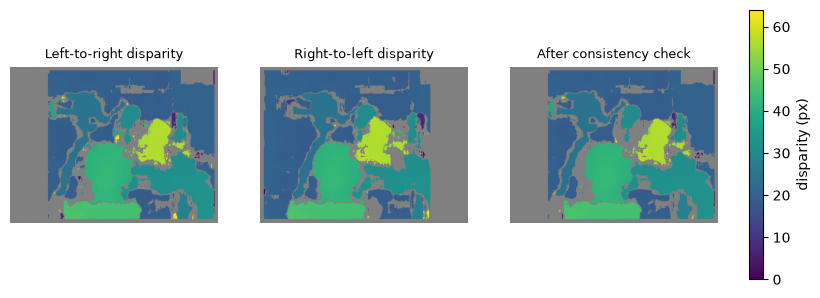
\includegraphics[width=0.9\textwidth]{figures/lesson22_fig08.png}
\caption{Left-to-right, right-to-left, and consistency-checked disparity on the Tsukuba stereo pair. The lamp, the nearest object in the scene, stands out with the largest disparity; the bookshelves recede smoothly behind it. Only $1121$ of $110{,}592$ pixels ($1.0\%$) get flagged --- concentrated exactly along depth discontinuities: book spines, shelf edges, the head's silhouette. \attrib{Image source: \href{https://vision.middlebury.edu/stereo/data/scenes2001/}{Middlebury Stereo Datasets} (University of Tsukuba).}}
\label{fig:l22-6}
\end{figure}

\section{From disparity to depth map}

Given a focal length and baseline (in whatever consistent units), $Z=fB/d$ converts a disparity map directly into a metric depth map (Figure~\ref{fig:l22-7}), which can then be lifted into a 3D point cloud (Figure~\ref{fig:l22-8}).

\begin{figure}[h]
\centering
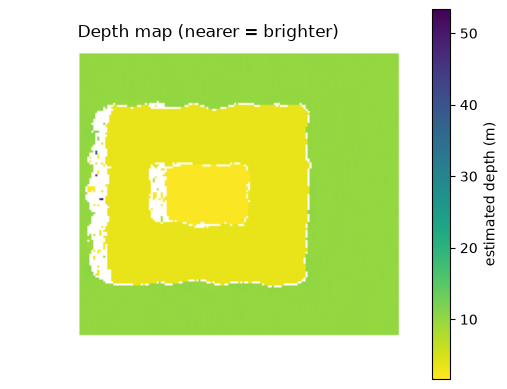
\includegraphics[width=0.45\textwidth]{figures/lesson22_fig09.png}
\caption{The synthetic scene's disparity map converted to metric depth.}
\label{fig:l22-7}
\end{figure}

\begin{figure}[h]
\centering
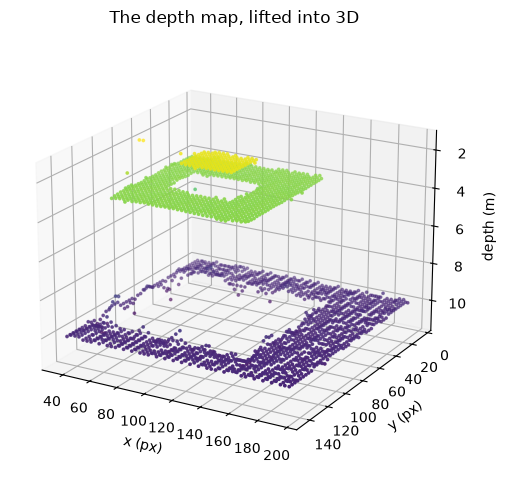
\includegraphics[width=0.55\textwidth]{figures/lesson22_fig10.png}
\caption{The depth map lifted into 3D: three flat terraces at three different heights, with holes where \code{StereoBM} had no confident match cut cleanly out of each one.}
\label{fig:l22-8}
\end{figure}

\subsection*{Exercises}
\begin{enumerate}
  \item Replace the random-texture left image with a flat gray region for the background (keeping the two rectangles textured). Run \code{cv2.StereoBM} again and describe what happens to the disparity estimate over the flat area --- this is the aperture problem from Chapter~\ref{ch:lesson21}, now in a stereo-matching context.
  \item Try \code{cv2.StereoSGBM\_create} (semi-global block matching, which enforces smoothness across neighboring disparities rather than matching each pixel completely independently) in place of \code{StereoBM}. Compare the amount of speckle noise in flat/background regions between the two methods.
  \item Increase the baseline in the depth conversion. How does the estimated depth map change, and why would a wider-baseline stereo rig give more precise depth estimates for distant objects (at the cost of a larger minimum-distance blind spot near the cameras)?
\end{enumerate}

\vfill
\fullcode{lesson22}{lesson22_stereo_matching}
